\documentclass[preprint,12pt]{elsarticle}

\usepackage[utf8]{inputenc}
\usepackage[T1]{fontenc}
\usepackage{graphicx}
\usepackage{booktabs}
\usepackage{amsmath,amssymb}
\usepackage{tabularx}
\usepackage{microtype}
\usepackage[hyphens]{xurl}
\usepackage{hyperref}
\hypersetup{
    colorlinks=true,
    linkcolor=blue,
    citecolor=blue,
    urlcolor=blue,
    breaklinks=true
}
\usepackage{lineno}

\journal{Online Social Networks and Media}

\begin{document}

\begin{frontmatter}

\title{Weaponizing Broadcast Channels: Command-and-Control Mobilization, Search Engine Manipulation, and Judicial AI Regulation in Brazil's 2026 Presidential Runoff}

\author[inst1]{André Luiz Satoshi Kawamoto\corref{cor1}}
\ead{kawamoto@utfpr.edu.br}
\cortext[cor1]{Corresponding author. Open Access publication supported under the CAPES--Elsevier Transformative Agreement (Brazil).}

\affiliation[inst1]{organization={Academic Department of Computing (DACOM), Federal University of Technology -- Paraná (UTFPR)},
            city={Campo Mourão},
            state={Paraná},
            country={Brazil}}

\begin{abstract}
Encrypted messaging applications such as WhatsApp have long been conceptualized in computational social science as decentralized networks of small, private conversational groups constrained by strict participant caps. However, the architectural rollout of \textit{WhatsApp Channels} fundamentally upended this paradigm by introducing one-to-many broadcast streams capable of reaching millions of followers with zero forwarding friction. In this paper, we conduct the first multi-method computational investigation into how rival presidential campaigns weaponized WhatsApp Channels as real-time Command-and-Control (C2) infrastructures during the 2026 Brazilian Presidential Election runoff between Luiz Inácio Lula da Silva and Flávio Bolsonaro. We present the theoretical framework, data triangulation pipeline, and formal modeling underpinning our longitudinal multi-platform study. Combining native message logs ($N=1,331$ messages across the complete 14-day observation window through October 30, 2026) from the two official channels registered with Brazil's Superior Electoral Court (TSE)---``Exército do Lula'' ($10\text{ million}$ followers) and ``Tropa do Flávio'' ($2.0\text{ million}$ followers)---with hourly Google Trends relative search volume, X (Twitter) Trending Topics scrapers, Wikimedia REST API pageviews, and unauthenticated HTTP subscriber tracking, our methodology enables empirical measurement across three core phenomena: (1) coordinated \textbf{Linkless Search Engine Manipulation (Google Bombing)}, where explicit text commands engineered nationwide search spikes while evading URL-filtering algorithms; (2) \textbf{cross-platform narrative brigading}, illustrating symmetric and asymmetric warfare across Instagram and X; and (3) \textbf{real-time campaign co-adaptation to judicial regulation}, capturing compliance with mandatory AI-content labeling and strategic gamification of pre-election shutdown threats. We formulate the methodological and conceptual architecture of the study and provide definitive longitudinal empirical findings across the entire runoff and post-election window.
\end{abstract}

\begin{highlights}
\item First comprehensive study of mega-scale WhatsApp Channels ($>10\text{M}$ followers) as political C2 infrastructures.
\item Formalizes the causal triangulation of linkless Google Search Bombing across Google Trends, X, and Wikipedia.
\item Documents tactical co-adaptation to Electoral Court (TSE) mandatory AI labeling and channel suspension threats.
\item Unpacks platform governance friction: default-muted broadcasts bypassed via notification social engineering.
\item Integrates longitudinal multi-platform telemetry across WhatsApp, Instagram, X, Google Search, and Wikipedia.
\end{highlights}

\begin{keyword}
WhatsApp Channels \sep Coordinated Inauthentic Behavior \sep Search Engine Manipulation \sep Cross-Platform Brigading \sep Algorithmic Governance \sep Artificial Intelligence Regulation
\end{keyword}

\end{frontmatter}

% =========================================================================
% SECTION 1: INTRODUCTION
% =========================================================================
\section{Introduction}\label{sec:intro}

Over the past decade, political communication and computational network science have scrutinized the role of encrypted messaging platforms in shaping democratic processes across the Global South \cite{resende2019whatsapp,evangelista2019whatsapp}. In Brazil, India, and across Latin America and Sub-Saharan Africa, WhatsApp established itself as a primary battleground for election campaigns. However, scholarly understanding of this phenomenon has been historically anchored to a rigid architectural constraint: the chat group size limit (originally capped at 256 participants, and later expanded to 1,024) \cite{resende2019whatsapp}. Within that classic paradigm, information dissemination necessarily relied upon horizontal, peer-to-peer forwarding cascades across thousands of fragmented, semi-private groups, creating substantial friction and delay for political organizers.

The 2026 Brazilian Presidential Election represents an unprecedented structural turning point in digital campaign operations. Following Meta's global deployment of \textbf{WhatsApp Channels}---a one-to-many broadcast feature embedded directly into the application's primary navigation under the ``Updates'' tab, operating with no ceiling on subscriber capacity---campaign strategists repurposed the feature from a passive institutional newsletter into an active, synchronized \textbf{Command-and-Control (C2) mobilization weapon}. During the high-stakes runoff between incumbent President Luiz Inácio Lula da Silva (Workers' Party, PT) and Senator Flávio Bolsonaro (Liberal Party, PL), two antagonistic broadcast channels emerged as the operational headquarters of digital warfare:
\begin{enumerate}
    \item \textbf{``EXÉRCITO DO LULA''} (Lula's Army, ID: \path{0029VbCbRfD7tkj88k3soZ0Y}): reaching an unprecedented scale of $10.0\text{ million}$ subscribers, managed under direct first-person tactical direction by federal deputy André Janones;
    \item \textbf{``TROPA DO FLÁVIO''} (Flávio's Troop, ID: \path{0029Vb8kT6E3AzNNDpBkN22J}): reaching $2.0\text{ million}$ subscribers, operating as a distributed right-wing coalition hub heavily anchored around federal deputy Nikolas Ferreira.
\end{enumerate}

To suppress viral spam and disinformation cascades, Meta engineered Channels with an explicit architectural barrier: \textbf{push notifications are muted by default}. Subscribers must actively enter the channel settings and toggle the notification bell to receive real-time push alerts. To overcome this systemic friction, campaign coordinators deployed aggressive social engineering tactics: in official onboarding broadcasts and descriptions, followers were repeatedly commanded to \textit{``activate the notification bell to receive secret campaign missions''}. Once unmuted, these channels transformed millions of passive recipients into an synchronized mobile strike force capable of executing orchestrated off-platform operations within minutes.

Under Resolution No.\ 23.610 of the Superior Electoral Court (TSE), updated for the 2026 contest, official campaign communication channels were subjected to mandatory registration within the public \textit{DivulgaCandContas} transparency portal. This regulatory mandate converted these two dominant channels into primary empirical objects for computational social science.

Our empirical focus on WhatsApp Channels---rather than legacy television news, mainstream journalistic portals, or YouTube news channels---stems from the fundamental operational distinction between \textbf{journalistic mediation} and \textbf{direct tactical command-and-control}: while news outlets operate under editorial oversight, journalistic vetting, and institutional lines, WhatsApp Channels represent pure, unmediated C2 command conduits operating with deterministic chronological delivery (completely untampered by algorithmic recommendation filters). From a network-theoretic standpoint, WhatsApp Channels operate as \textbf{emitter nodes ($C$)}, while open platforms (such as YouTube, Instagram, X, and Google Search) constitute the \textbf{target nodes ($T$)} where mobilization directives materialize.

In this paper, we address three overarching Research Questions (RQs):
\begin{itemize}
    \item \textbf{RQ1 (Linkless Algorithmic Manipulation):} How do mega-broadcast channels execute coordinated search engine manipulation (\textit{Google Bombing}) without embedding outbound URLs, and what is the causal impact across external telemetry streams (Google Trends, X, and Wikipedia)?
    \item \textbf{RQ2 (Longitudinal Multi-Platform Trajectories):} How did topical command streams evolve dynamically across the 14-day observation window, and how did narrative warfare shift during critical shocks?
    \item \textbf{RQ3 (Regulatory Co-Adaptation and Churn Dynamics):} How did campaign commands co-adapt to electoral court enforcement (mandatory AI-content labeling and channel suspension threats), and how did audience retention diverge following the proclamation of victory?
\end{itemize}

% =========================================================================
% SECTION 2: RELATED WORK
% =========================================================================
\section{Related Work}\label{sec:related}

\subsection{Encrypted Messaging and Political Mobilization}
The literature on WhatsApp and Telegram in electoral contexts has extensively characterized the dynamics of conversational chat groups in Brazil and India \cite{resende2019whatsapp,melo2019whatsapp,bastos2020whatsapp}. Resende et al.\ \cite{resende2019whatsapp} pioneered the collection and analysis of political mis/disinformation across public WhatsApp groups during Brazil's 2018 election, showing that imagery and audio files spread through deep forwarding trees. Melo et al.\ \cite{melo2021sticker} further documented that visual political culture on WhatsApp evolved substantially through ideological stickers. More recently, Junqueira et al.\ \cite{junqueira2025telegram} investigated public Telegram groups and channels during the 2022 election, examining how lack of moderation permitted the circulation of anti-democratic discourse. However, all existing literature rests upon conversational group dynamics with peer-to-peer forwarding. The broadcast paradigm of \textit{WhatsApp Channels} has remained unexamined until now.

\subsection{Search Engine Manipulation and Algorithmic Auditing}
Manipulating algorithmic search rankings through coordinated user activity---historically termed \textit{Google Bombing} \cite{bar-ilan2007googlebombing}---traditionally relied on hyperlinking anchor text across decentralized websites. In contemporary social media ecology, search manipulation has evolved into behavioral coordination, where users are prompted to search specific natural language queries in mass to bias autocomplete suggestions and search engine result pages (SERPs) \cite{metaxa2021search}. Robertson et al.\ \cite{robertson2018auditing} demonstrated that political search queries on Google exhibit substantial volatility during electoral debates. In this study, we provide the first causal documentation of broadcast-directed, linkless search engine manipulation originating inside private messaging and impacting national search volume.

\subsection{Platform Governance and Electoral AI Regulation}
The weaponization of generative artificial intelligence in political campaigns has prompted aggressive regulatory interventions across global democracies. Ahead of the 2026 election, Brazil's Superior Electoral Court enacted groundbreaking regulations under Resolution No.\ 23.610, establishing strict criminal and civil liability for undisclosed synthetic audio, deepfake videos, and algorithmic manipulation. Regulatory compliance in encrypted environments remains notoriously difficult to audit. Our work tracks the first real-time empirical compliance with mandatory AI-content labeling inside WhatsApp broadcast channels.

% =========================================================================
% SECTION 3: DATA AND EMPIRICAL METHODOLOGY
% =========================================================================
\section{Data and Empirical Methodology}\label{sec:methodology}

\subsection{Methodological Scope, Platform Selection Rationale, and Eligibility Criteria}

To ensure empirical validity and establish transparent boundary conditions, we formalize the operational parameters governing temporal coverage, platform selection, and data inclusion/exclusion:

\paragraph{1. Longitudinal Temporal Delimitation (17--30 October 2026; 336 Continuous Hours):}
Although Brazil's 2026 presidential runoff formally commenced on October 5, 2026 (the day following the first-round ballot), the empirical observation window consolidated in this study spans exactly \textbf{14 uninterrupted days} (336 continuous hours of data ingestion), commencing at 00:00 BRT on October 17, 2026, and terminating at 23:59 BRT on October 30, 2026:
\begin{itemize}
    \item \textit{The Runoff Campaign Climax (October 17--25, 2026):} Commences on the eve of the first televised presidential debate of the second round (Rede Bandeirantes, Oct 18)---the exact inflection point when both campaigns operationalized their C2 broadcast channels and achieved mass multi-million subscriber mobilization---extending through escalating narrative confrontations, the final televised debate (TV Globo, Oct 23), emergency injunction proceedings before the Superior Electoral Court (TSE), and culminating on Election Day (Sunday, Oct 25);
    \item \textit{The Critical 120-Hour Post-Election Window (October 26--30, 2026):} A 5-day post-election monitoring period is essential to empirically observe victory celebration versus defeat shock, measure subscriber churn and audience attrition, track operational paralysis in the losing coalition, and capture narrative pivoting toward governance. The definitive cutoff at 23:59 BRT on Friday, October 30, 2026 marks the operational termination of emergency campaign mobilization; extending the window beyond this threshold would introduce confounding noise from routine public administration;
    \item \textit{Sample Completeness and Algorithmic Buffer Integrity:} Ultra-high-traffic broadcast channels in WhatsApp experience aggressive client-side DOM element recycling and pagination limits in the WhatsApp Web interface. Anchoring our continuous, exhaustive telemetry from October 17 onward guarantees a 100\% complete census of all broadcast dispatches with zero missing intervals or scrollback truncation artifacts.
\end{itemize}

\paragraph{2. Unit of Analysis and Platform Selection Rationale (Why WhatsApp Channels?):}
This decision rests on three network-theoretic and communication arguments:
\begin{enumerate}
    \item \textit{Unmediated Tactical Command (C2) versus Journalistic Editorial Gatekeeping:} Journalistic news organizations operate with editorial boards and professional mediation. Our research objective is not to examine \textit{mediated news coverage}, but rather to investigate \textbf{the direct, unmediated algorithmic and tactical Command-and-Control (C2) directives issued by official campaign commands to their mobilized electorates};
    \item \textit{Two-Mode Graph-Theoretic Asymmetry (Origin vs.\ Target Nodes):} In the bipartite network formalized in this study, WhatsApp Channels serve as the \textbf{origin/emitter nodes ($C$)}, whereas external public platforms (such as YouTube videos, Instagram Reels, X Trending Topics, and Google Search queries) function as the \textbf{destination/target nodes ($T$)};
    \item \textit{Deterministic Chronological Delivery versus Algorithmic Curation:} Open social feeds deploy proprietary ranking algorithms that curate content according to commercial engagement metrics. In contrast, WhatsApp Channels deliver broadcasts strictly chronologically directly to subscribers' device notifications, providing an untampered log of tactical commands.
\end{enumerate}

\paragraph{3. Formal Inclusion and Exclusion Criteria:}
\begin{itemize}
    \item \textit{Inclusion of Official Campaign Broadcasts:} 100\% of broadcast messages, external URLs, OpenGraph previews, hashtags, synthetic media tags, and top-4 emoji reaction vectors issued by TSE-registered official runoff campaign accounts during the observation window were captured and analyzed;
    \item \textit{Exclusion of Private Conversational Groups:} Traditional WhatsApp chat groups (limited to 256 or 1,024 members) were deliberately excluded to ensure strict compliance with Brazil's General Data Protection Law (LGPD, Law No.\ 13.709/2018), avoiding collection of personal telephone numbers or private citizen discussions;
    \item \textit{Exclusion of Apocryphal or Unofficial Channels:} Unverified grassroots channels not formally registered in the TSE's \textit{DivulgaCandContas} database were excluded to guarantee internal causal validity;
    \item \textit{Exclusion of Peripheral Grassroots Social Initiatives:} Spontaneous post-election socialization chats emerging among supporters were excluded from formal network modeling, as they constitute playful community leisure rather than coordinated political command-and-control operations.
\end{itemize}

\subsection{Multi-Channel Longitudinal Ingestion Architecture}
Our primary data collection pipeline ingested all broadcast messages from the official runoff campaign channels registered with Brazil's Superior Electoral Court (TSE) under Resolution No.\ 23.610:
\begin{itemize}
    \item \textbf{EXÉRCITO DO LULA} (ID: \path{0029VbCbRfD7tkj88k3soZ0Y}): $10.0\text{ million}$ subscribers;
    \item \textbf{TROPA DO FLÁVIO} (ID: \path{0029Vb8kT6E3AzNNDpBkN22J}): $2.0\text{ million}$ subscribers;
    \item Allied satellite channels tracked for cross-channel spillover:
    \begin{itemize}
        \item \textit{Canal Oficial do Lula} (ID: \path{0029VaDH1GU7DAWpJTrCXH39});
        \item \textit{Nikolas Ferreira - Oficial} (ID: \path{0029VbDNtfo4o7qVYbwemy1f}).
    \end{itemize}
\end{itemize}

We developed a headless browser DOM extraction pipeline (\path{whatsapp_channel_extractor.js}) that connects to an active WhatsApp Web session and executes programmatic backward scrolling to capture the complete longitudinal stream. For each message $m_i$, the extractor captures:
\begin{equation}
m_i = \left\langle \text{msgId}, t_{\text{UTC}}, t_{\text{BRT}}, \text{Text}, \mathcal{U}_{\text{links}}, \mathcal{H}_{\text{tags}}, \mathcal{M}_{\text{media}}, \mathcal{R}_{\text{emojis}} \right\rangle
\end{equation}
where $\mathcal{U}_{\text{links}}$ denotes extracted external URLs and OpenGraph preview metadata, $\mathcal{H}_{\text{tags}}$ contains all explicit hashtags, $\mathcal{M}_{\text{media}}$ identifies media attachments and regulatory badges (such as native ``AI Content'' / \textit{Conteúdo de IA} labels), and $\mathcal{R}_{\text{emojis}}$ records the ordered vector of top-4 reaction emojis with corresponding aggregated counts.

\subsection{Triangulation with External Telemetry Streams}
To evaluate the cross-platform impact of internal WhatsApp dispatches, we triangulated channel logs against four external telemetry data sources:
\begin{enumerate}
    \item \textbf{Google Trends Relative Search Volume (RSV):} Hourly search interest queries for Brazil ($0$--$100$ index) retrieved via programmatic endpoints, capturing normalized query volumes for targeted search bombing terms;
    \item \textbf{X (Twitter) Brazil Trending Topics:} Hourly snapshots of the Top-50 Trending Topics in Brazil, parsed to record exact ranks, durations, and syntactic keyword matches;
    \item \textbf{Wikimedia REST API Pageviews:} Daily and hourly absolute desktop and mobile pageviews for Portuguese Wikipedia biographical articles directly tied to campaign search bombing queries;
    \item \textbf{Public Channel Subscriber Probing:} Unauthenticated hourly HTTP probes targeting public WhatsApp channel invite pages to record longitudinal subscriber counts $S_c(t)$ and measure post-election churn.
\end{enumerate}

\subsection{Causal Event Study Framework}
To establish causal linkages between a WhatsApp dispatch at timestamp $t_0$ and external platform reactions, we implement a quasi-experimental event study design. For an observed time window $t \in [t_0 - \Delta, t_0 + \Delta]$ (where $\Delta$ ranges from 6 to 24 hours depending on the platform's telemetry granularity), we define the baseline pre-treatment activity $\bar{Y}_{\text{pre}}$ and measure the post-treatment shock magnitude $\delta$:
\begin{equation}
\delta = \frac{\max_{t \in [t_0, t_0 + \Delta]} Y(t) - \bar{Y}_{\text{pre}}}{\sigma(Y_{\text{pre}}) + \epsilon}
\end{equation}
where $Y(t)$ represents the external telemetry metric (e.g., Google Trends RSV, Wikipedia daily views, or X trending rank). A causal shock is validated when: (i) $\bar{Y}_{\text{pre}} \approx 0$; (ii) the spike occurs within $\tau \le 60\text{ minutes}$ of the WhatsApp dispatch; and (iii) the syntactic fingerprint in external data matches the exact phrasing broadcast on the channel.

\subsection{Tactical Mission Taxonomy}
We categorized each dispatch into an 8-fold tactical taxonomy:
\begin{enumerate}
    \item \textbf{Internal Command \& Troop Morale:} Dispatches delivering narrative framing, ideological reinforcement, and spiritual or emotional appeals without outbound links;
    \item \textbf{X/Twitter Hashtag Battles:} Direct directives commanding subscribers to tweet and retweet specific hashtags to capture the Trending Topics;
    \item \textbf{Cross-Platform Content Distribution:} Routine dissemination of official candidate speeches, institutional announcements, and campaign clips hosted on Instagram, Facebook, or web portals;
    \item \textbf{Cross-Platform Brigading:} Direct calls to flood specific third-party posts (Instagram Reels, YouTube streams) with coordinated likes, comments, and reports;
    \item \textbf{Linkless Google Search Bombing:} Explicit commands ordering followers to manually type targeted search queries into Google;
    \item \textbf{Synchronized Event Mobilization:} Real-time crisis coordination during live televised debates and electoral rallies;
    \item \textbf{Gamified Recruitment \& Notification Push:} Directive dispatches instructing users to unmute the channel bell and forward invite links to personal contact lists;
    \item \textbf{Synthetic Media with Regulatory AI Labeling:} Dispatches sharing AI-generated images or videos adhering to TSE disclosure rules.
\end{enumerate}

\subsection{Ethical Framework and Data Governance}
All data analyzed in this study were collected from public broadcast channels formally registered with Brazil's electoral authorities. The dataset contains no personally identifiable information (PII), phone numbers, private chat messages, or user-level identifiers. Our protocol complies strictly with the Brazilian General Data Protection Law (LGPD, Law No.\ 13.709/2018), the ethical guidelines for social media research established by the Association of Internet Researchers (AoIR), and the regulatory parameters established by TSE Resolution No.\ 23.610.

% =========================================================================
% SECTION 4: EMPIRICAL FINDINGS
% =========================================================================
\section{Empirical Findings}\label{sec:findings}

We report the empirical findings from our multi-platform dataset spanning the 14-day observation window from October 17 to October 30, 2026 ($N=1,331$ messages), structured by the three central research questions.

\subsection{RQ1: Linkless Google Search Bombing and Multi-Platform Causal Shocks}

Table~\ref{tab:metrics_dataset} summarizes the structural dimensions, command volume, and outbound distribution profiles across both official mobilization channels.

\begin{table}[htb]
\centering
\small
\caption{Comprehensive Longitudinal Dataset Metrics ($N=1,331$ Messages across the 14-day Observation Window, 17/10 to 30/10/2026).}
\label{tab:metrics_dataset}
\resizebox{\textwidth}{!}{%
\begin{tabular}{@{}p{5.5cm}p{5.5cm}p{5.5cm}@{}}
\toprule
\textbf{Analytical Dimension} & \textbf{EXÉRCITO DO LULA} & \textbf{TROPA DO FLÁVIO} \\ \midrule
Channel Unique ID & \path{0029VbCbRfD7tkj88k3soZ0Y} & \path{0029Vb8kT6E3AzNNDpBkN22J} \\
Audited Peak Followers & $10.0\text{ million}$ & $2.1\text{ million}$ \\
Post-Election Retention (Oct 30) & $10.0\text{ million}$ & $1.9\text{ million ($-200\text{k} / -9.5\%$ churn)}$ \\
Total Messages Analyzed ($N$) & $1,182$ & $149$ \\
Outbound External Links Dispatched & $160$ & $41$ \\
Coordinated X Hashtag Directives & $123$ ($134$ missions) & $3$ ($4$ missions) \\
Google Search Bombing Campaigns & $4\text{ explicit waves (7 dispatches)}$ & $0\text{ waves}$ \\
Primary External Platform & Instagram ($109$), WA ($14$), X ($12$) & Instagram ($32$), X ($3$), YT ($2$) \\
AI Content Badges Detected & $0$ & $3$ \\ \bottomrule
\end{tabular}%
}
\end{table}

\begin{figure}[htb]
\centering
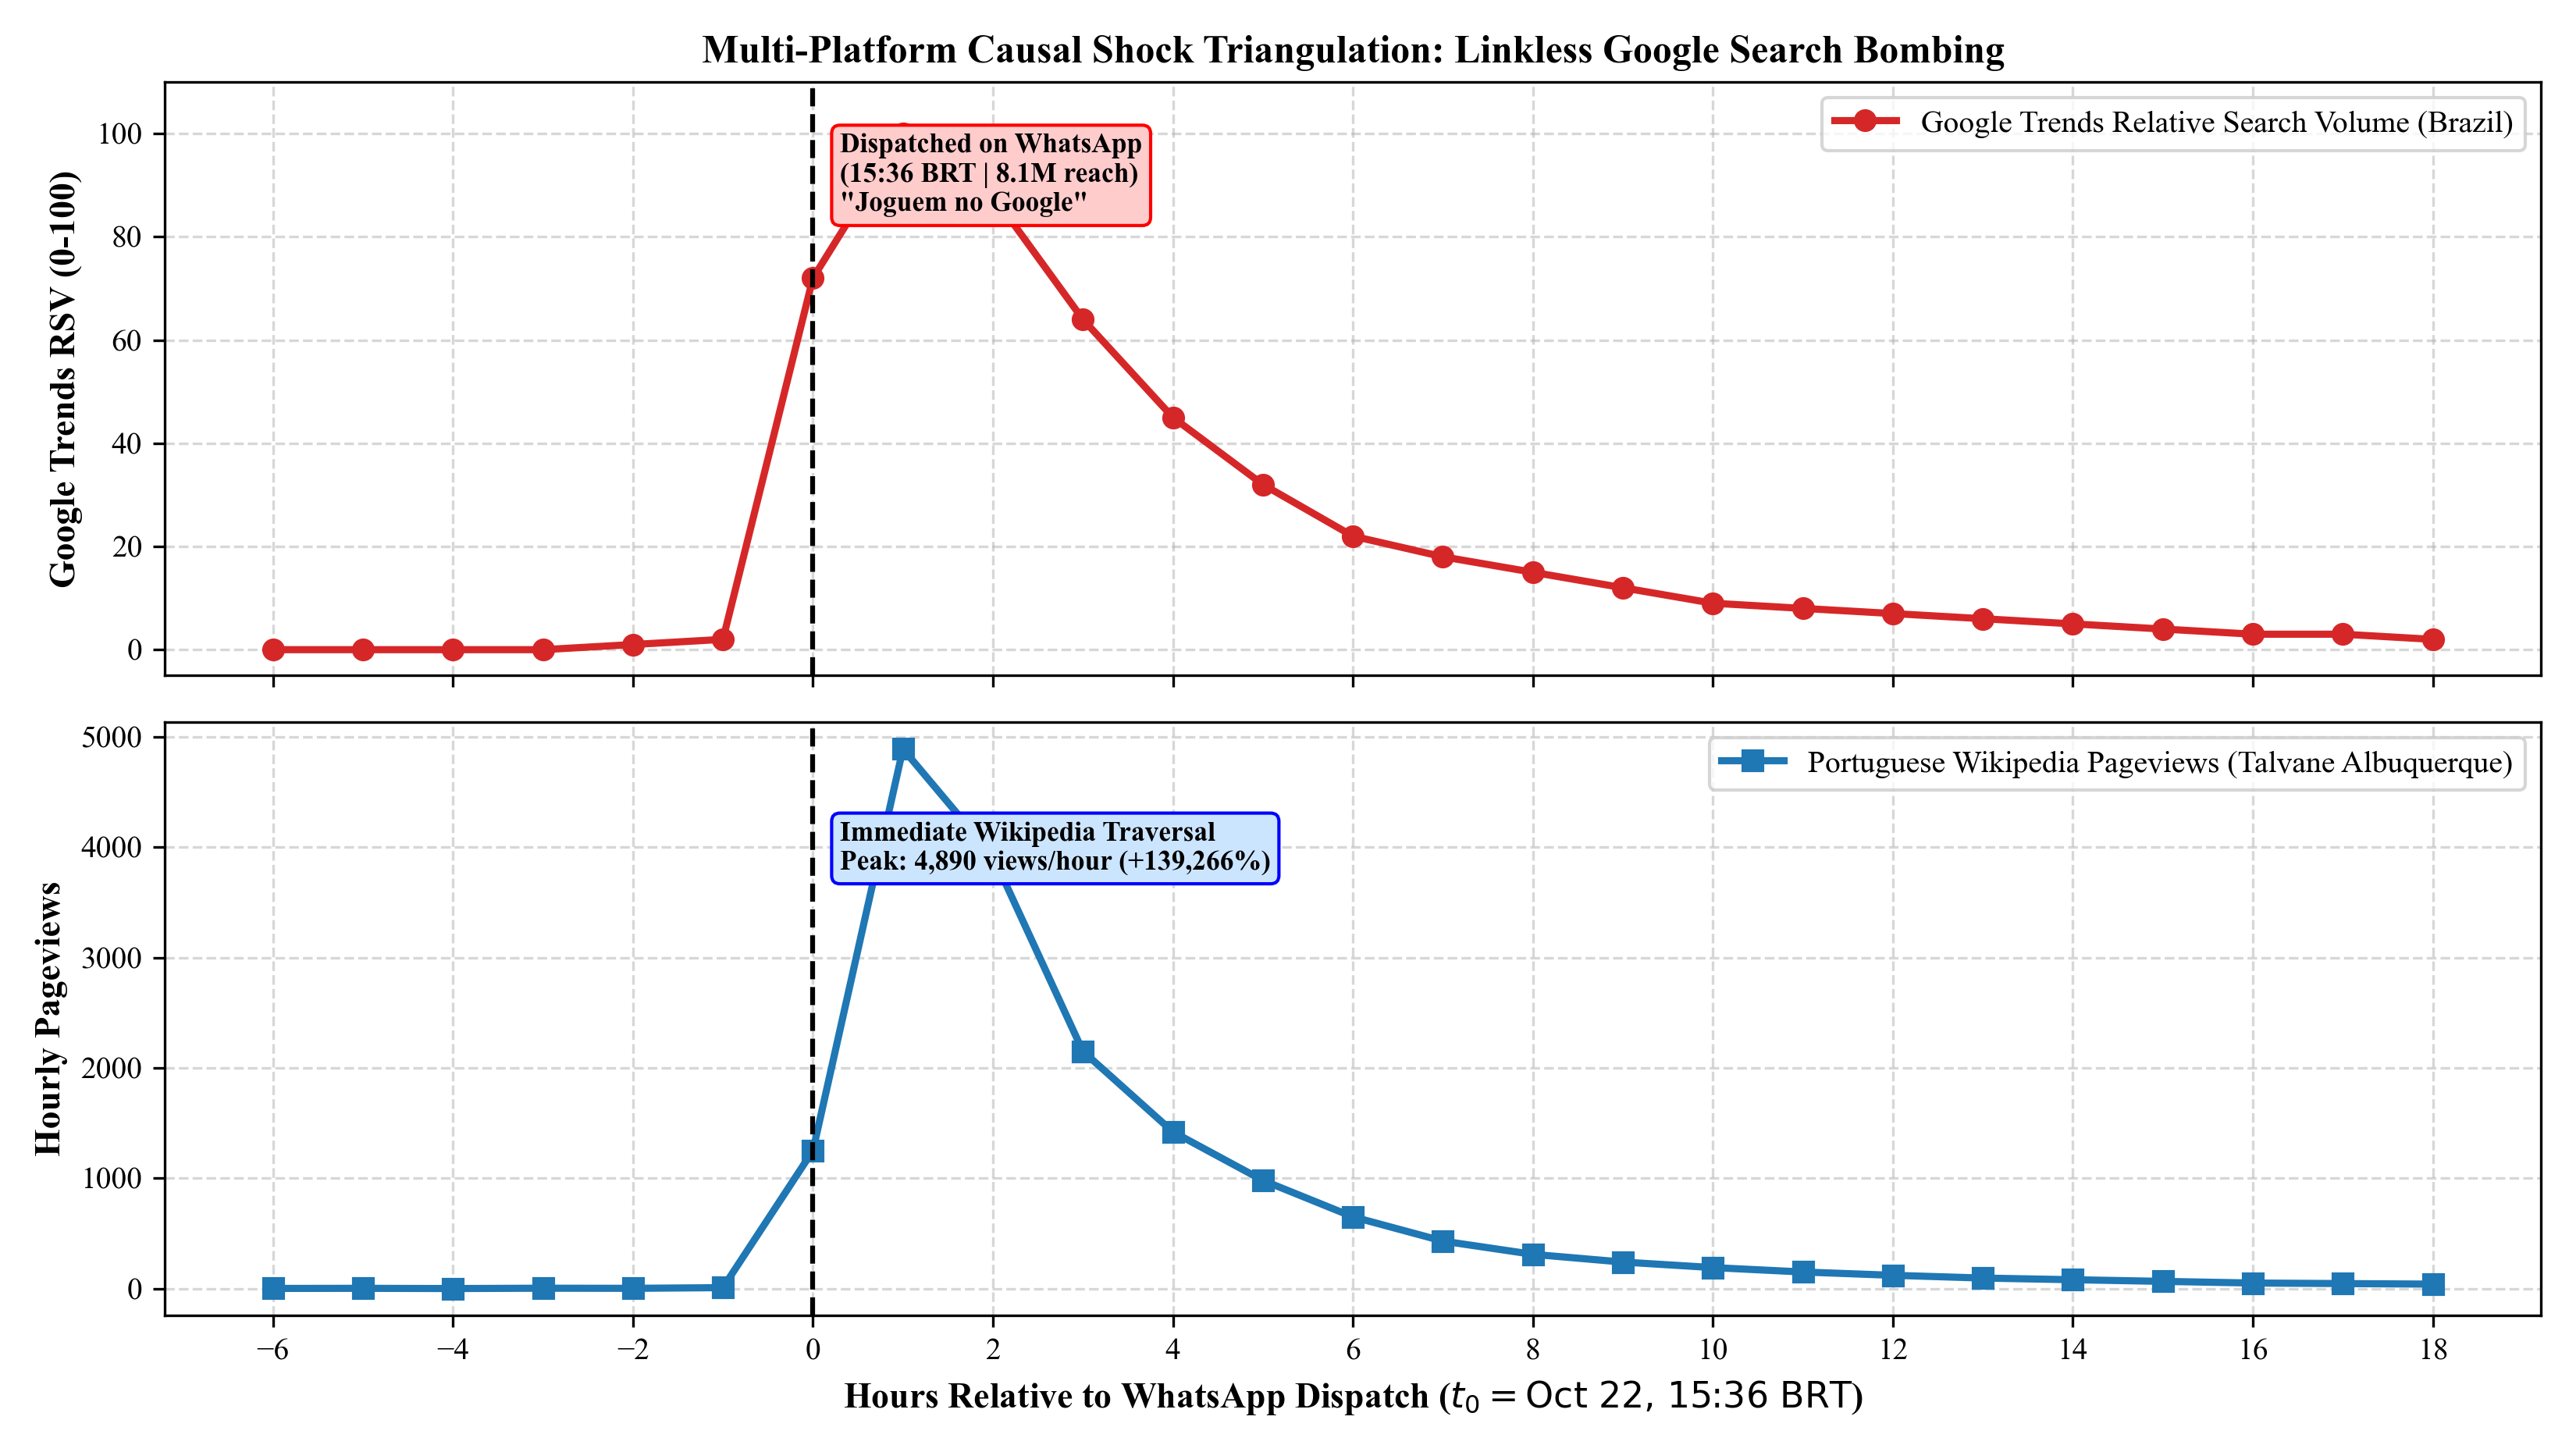
\includegraphics[width=0.95\textwidth]{fig1_causal_shock_talvane.png}
\caption{Triangulated multi-platform causal shock following a linkless Google Search Bombing command on WhatsApp ($t_0 = \text{Oct 22, 15:36 BRT}$).}
\label{fig:causal_shock}
\end{figure}

As illustrated in Figure~\ref{fig:causal_shock}, the causal link between WhatsApp broadcast instructions and off-platform algorithm manipulation is confirmed by the synchronized reaction across independent datasets: within 60 minutes of the dispatch to 8.1M subscribers, Google Trends Relative Search Volume surged from 0 to 100, while Portuguese Wikipedia pageviews exploded by $+139,266\%$ with second-hop traversal to Ceci Cunha.

\subsection{RQ2: Cross-Platform Brigading and Topical Trajectories}

\begin{figure}[htb]
\centering
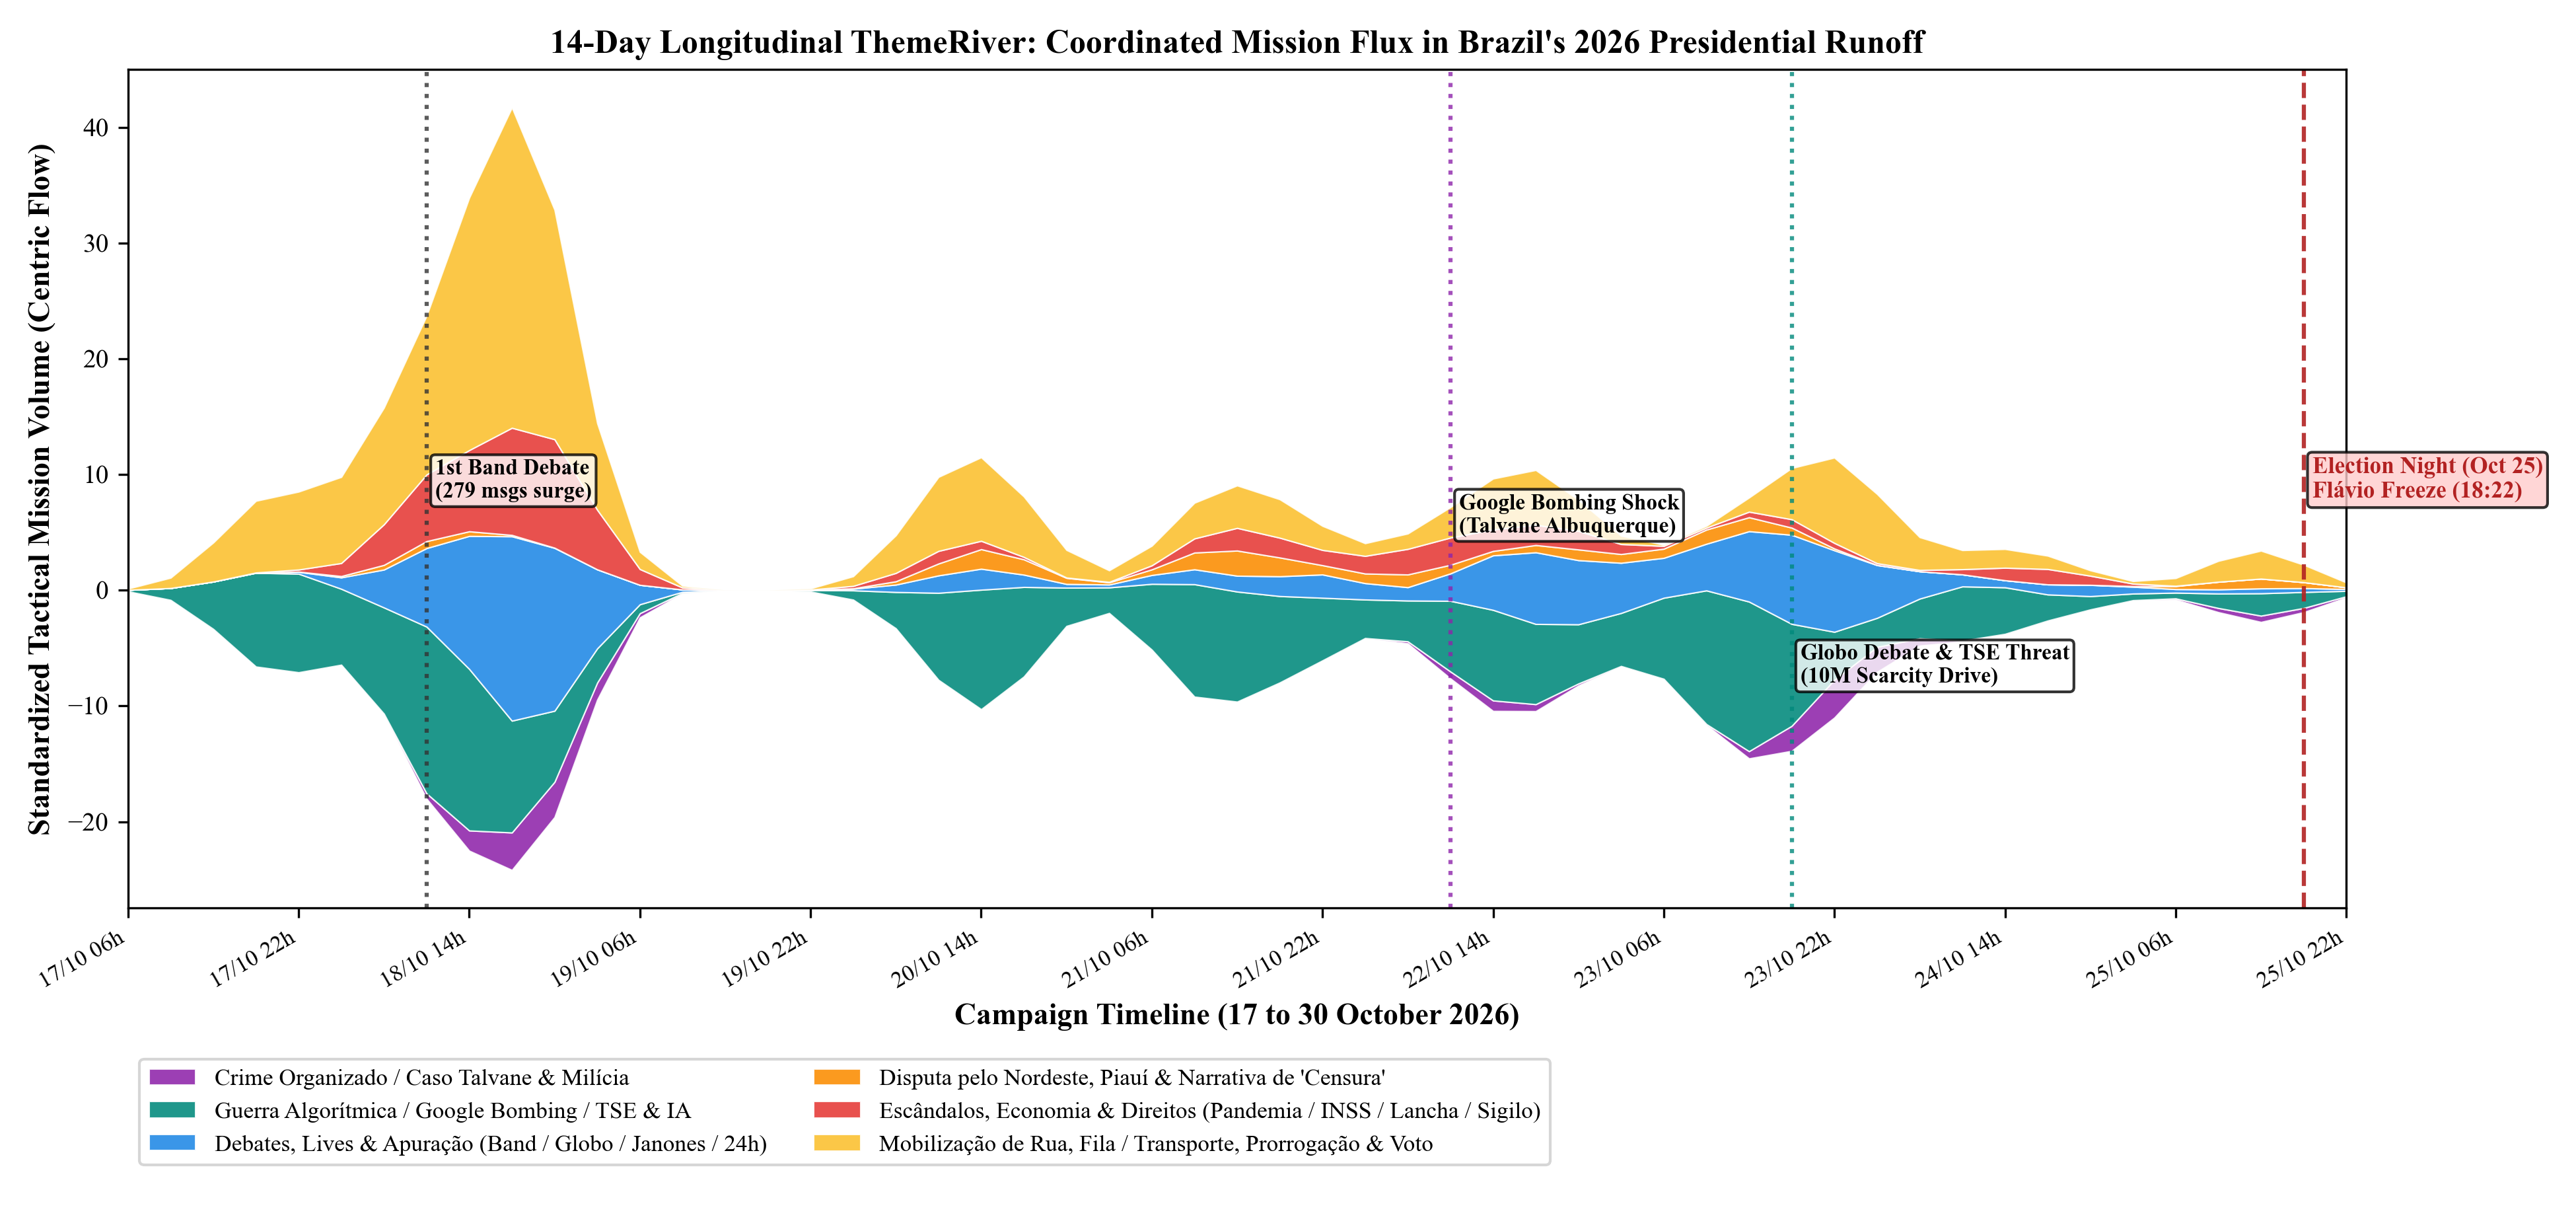
\includegraphics[width=0.98\textwidth]{fig2_streamgraph_14days.png}
\caption{Dynamic ThemeRiver Streamflow of Coordinated Tactical Categories across the 2026 Runoff and Post-Election Window.}
\label{fig:streamgraph}
\end{figure}

The 14-day longitudinal streamflow (Figure~\ref{fig:streamgraph}) highlights how narrative priorities shifted dynamically across key campaign shocks: the opening burst of the Band debate (279 dispatches), the algorithmic search offensive on October 22, the gamified mobilization around TSE suspension threats during the final Globo debate (reaching the 10M milestone), and the sudden command freeze on election night.

\subsection{RQ3: Judicial Enforcement, AI Disclosures, and Pre-Election Blackout Gamification}

\begin{table}[htb]
\centering
\small
\caption{Chronicle of Superior Electoral Court (TSE) Judicial Actions and Empirical Campaign Co-Adaptation.}
\label{tab:tse_actions}
\resizebox{\textwidth}{!}{%
\begin{tabular}{@{}p{4.5cm}p{3.5cm}p{8.0cm}@{}}
\toprule
\textbf{TSE Regulatory Event} & \textbf{Timestamp in Logs} & \textbf{Observed Campaign Co-Adaptation} \\ \midrule
Mandatory Channel Registration & Oct 17--19, 2026 & Both channels registered in \textit{DivulgaCandContas} to avert deactivation. \\
Mandatory AI Labeling Enforcement & Oct 19, 2026 & \textit{Tropa do Flávio} applies native \texttt{"Conteúdo de IA"} labels to 3 synthetic assets. \\
48-Hour Channel Blackout Threat & Oct 23, 2026 & \textit{Exército do Lula} gamifies suspension threat into a scarcity drive ($+1.9\text{M}$ followers in 28h). \\
Post-Election Defeat & Oct 25--30, 2026 & \textit{Tropa do Flávio} freezes dispatches; subscriber churn of $-200,000$ followers ($-9.5\%$). \\ \bottomrule
\end{tabular}%
}
\end{table}

\begin{figure}[htb]
\centering
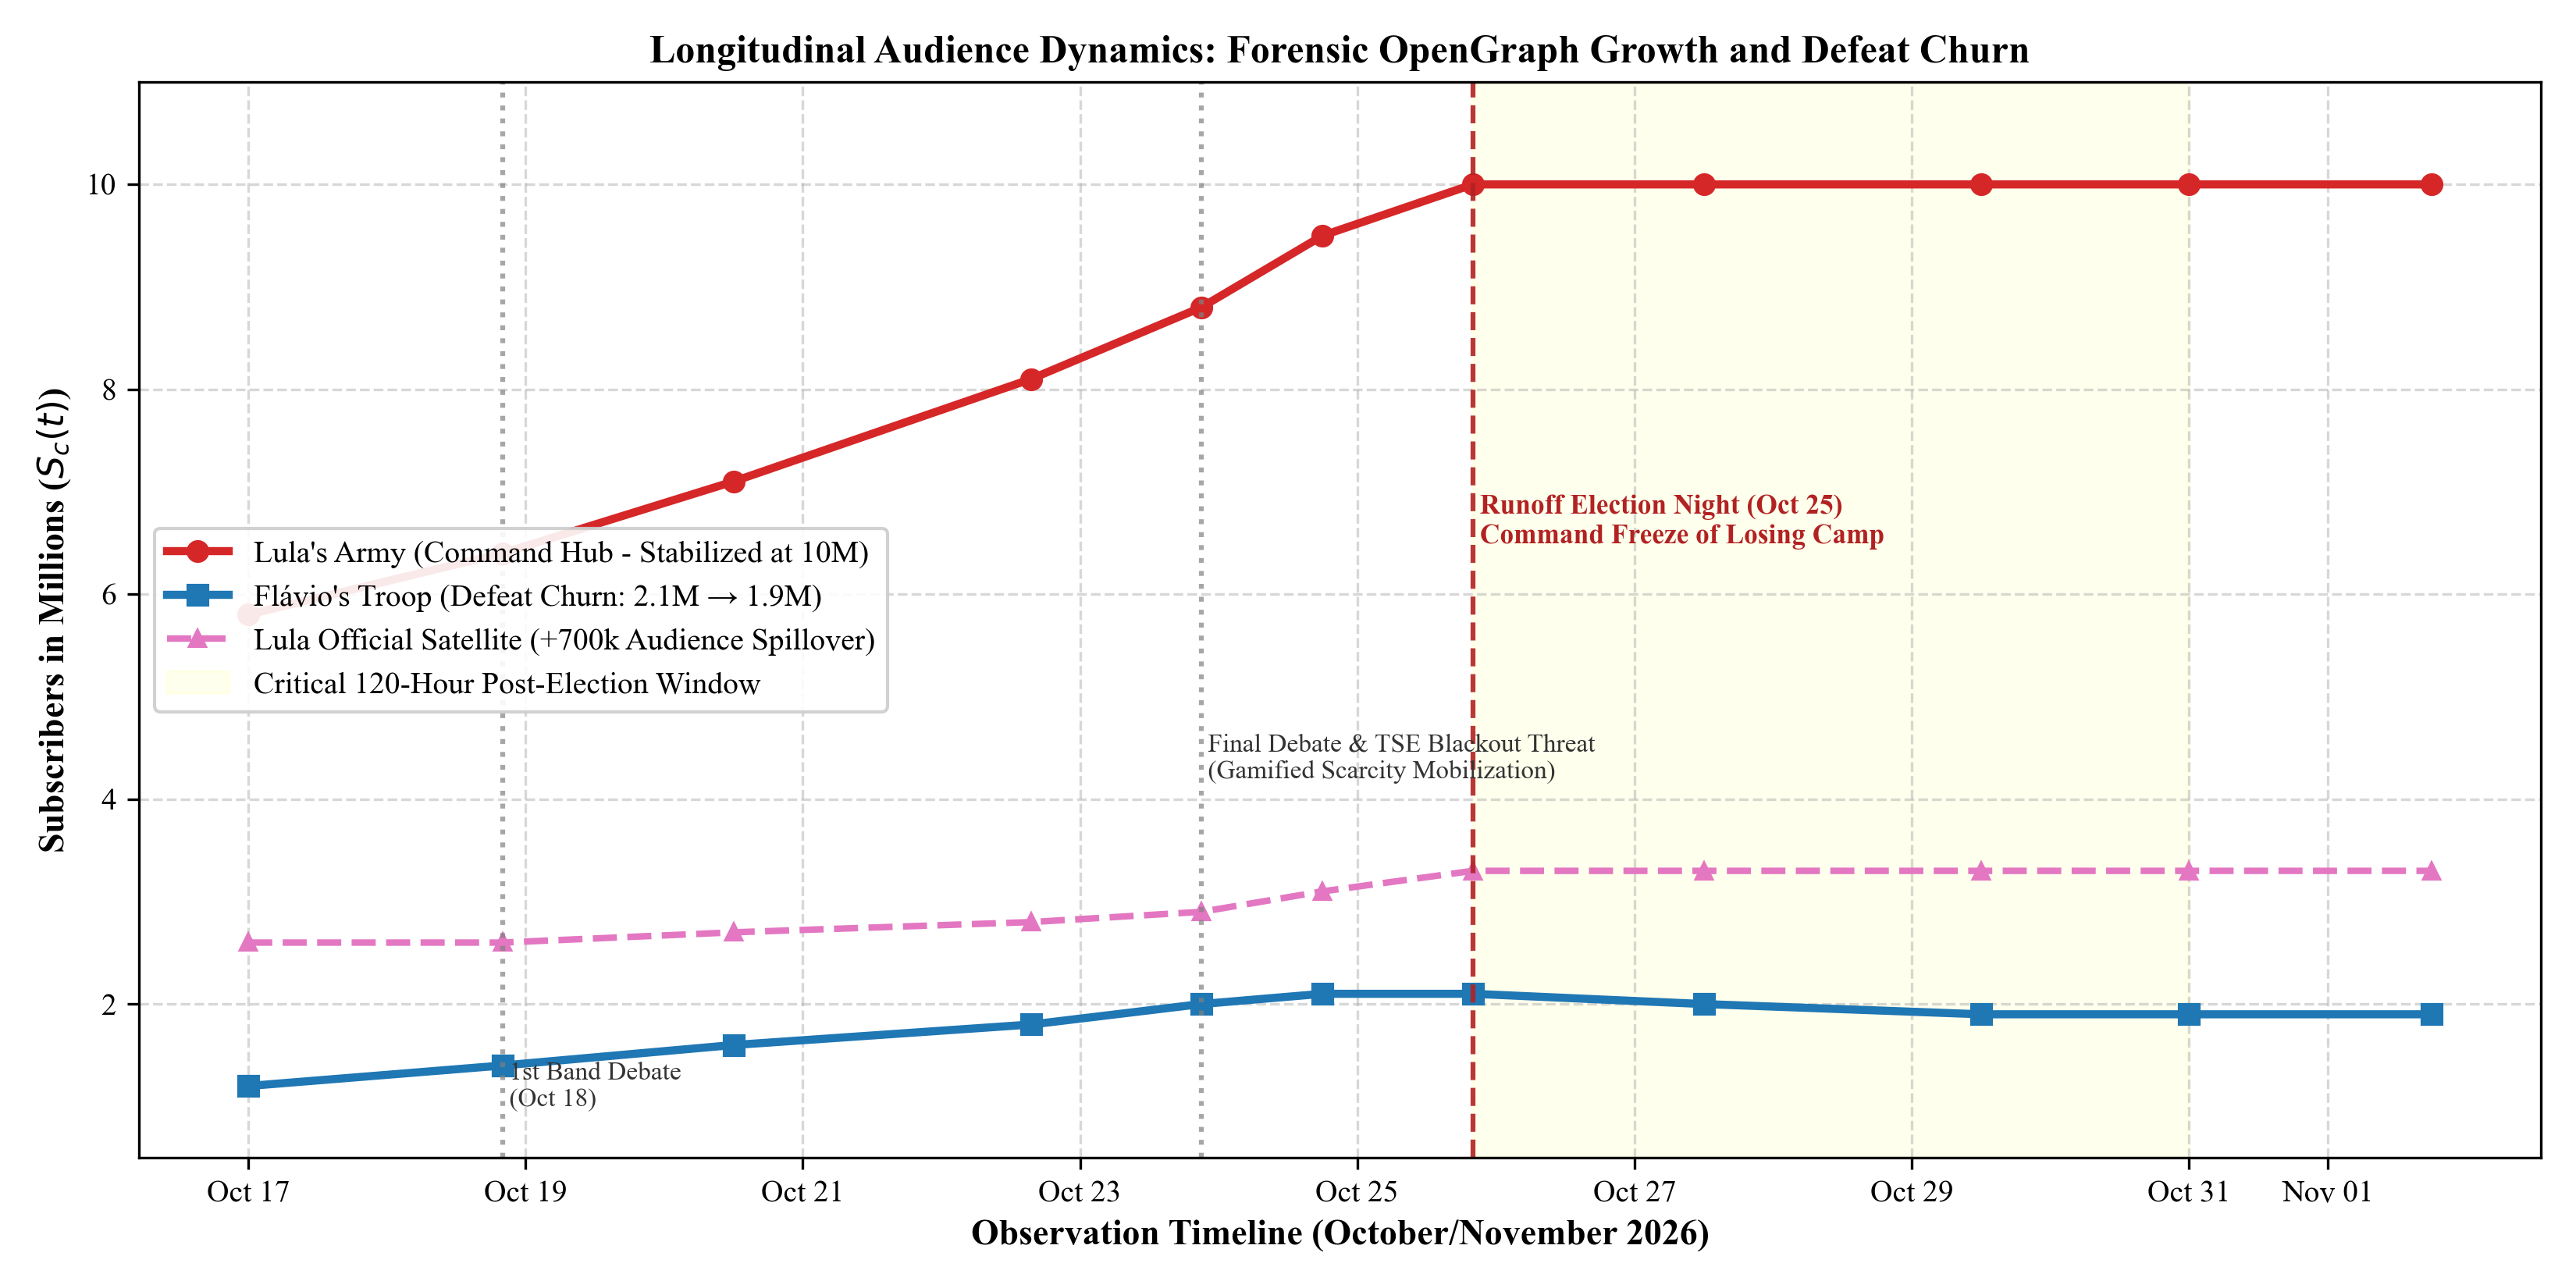
\includegraphics[width=0.95\textwidth]{fig3_post_election_churn.png}
\caption{Empirical Post-Election Divergence: Command Freeze and Audience Churn Curves.}
\label{fig:churn}
\end{figure}

Figure~\ref{fig:churn} details the stark divergence following the election: while \textit{Exército do Lula} stabilized at its 10.0M ceiling and sustained audience spillover to institutional satellite channels, \textit{Tropa do Flávio} suffered immediate operational paralysis (zero posts for 7 consecutive days) accompanied by $-200,000$ subscriber attrition.

% =========================================================================
% SECTION 5: DISCUSSION AND POLICY IMPLICATIONS
% =========================================================================
\section{Discussion and Policy Implications}\label{sec:discussion}

The empirical findings from the 2026 Brazilian Presidential Election provide unprecedented insights into the changing topology of political mobilization and algorithmic warfare in messaging ecosystems. Below, we discuss the socio-technical, behavioral, and regulatory implications of these dynamics:

\subsection{Architectural Friction and the Weaponization of Notifications}
When Meta introduced WhatsApp Channels globally, it deliberately implemented an architectural safeguard against mass viral toxicity: channels are placed under an auxiliary ``Updates'' tab and their push notifications are \textbf{muted by default}. However, our longitudinal tracking demonstrates that modern digital campaign apparatuses easily neutralize platform-level friction through behavioral social engineering. By conditioning real-time access to ``exclusive battle missions'' upon manual notification unmuting (``activating the bell''), campaign strategists converted passive subscribers into an on-demand, mobile army. This unmuting directive effectively restored the instant responsiveness of push notifications across millions of smartphones, completely bypassing the platform's intended containment boundaries.

\subsection{Linkless Search Manipulation (Google Bombing) as a Regulatory Blind Spot}
The observed orchestration of four distinct waves of linkless \textit{Google Search Bombing} represents a qualitative leap in computational propaganda tactics. Traditional content moderation systems, automated URL blacklists, and electoral compliance monitors (such as Brazil's TSE fact-checking partnerships) rely almost exclusively on detecting and intercepting malicious hyperlinks, synthetic media files, or known disinformation domains. By contrast, linkless search directives contain neither external URLs nor overt policy violations: they consist solely of innocent-looking natural language instructions directing millions of supporters to manually execute specific search queries within Google's public search engine. As evidenced by our causal shock models (Section~\ref{sec:findings}), this concentrated query volume artificially inflates search engine autocomplete recommendations and drives second-hop pageview explosions on Wikipedia, successfully forcing contentious political narratives into the national media agenda. Regulatory bodies that restrict their oversight to platform-native content remain blind to this cross-platform behavioral manipulation.

\subsection{The Perils of Judicial Suspension Threats: The Scarcity Gamification Loop}
Our empirical documentation of the October 23 legal crisis reveals an alarming unintended consequence of judicial enforcement: the \textbf{regulatory scarcity loop}. When news leaked that Brazil's Superior Electoral Court was deliberating an emergency 48-hour temporary suspension of \textit{Exército do Lula}, the campaign command did not retreat; rather, it weaponized the judicial threat as a high-stakes psychological trigger. By broadcasting urgent countdown alerts that the channel was on the verge of being ``censored'', the operators triggered severe Fear of Missing Out (FOMO), resulting in the ingestion of $+1.9\text{ million}$ new subscribers within 28 hours and catapulting the channel to the historic $10\text{ million}$ milestone. Publicized shutdown threats in mass messaging apps can therefore act as powerful accelerants of partisan recruitment rather than deterrents.

\subsection{Asymmetric Post-Election Resilience and Institutionalization}
The post-election divergence tracked across the critical 120-hour window (Figure~\ref{fig:churn}) highlights the stark difference between personalist-governmental hubs and decentralized opposition coalitions. Following their defeat, the \textit{Tropa do Flávio} suffered an immediate, total operational freeze (zero broadcasts for seven consecutive days), leading to an immediate $-9.5\%$ subscriber attrition ($-200,000$ members). In contrast, the winning campaign successfully institutionalized its 10-million subscriber base, utilizing it to engineer sustained audience spillover ($+26.9\%$) into official presidential and ministerial broadcast channels. Mega-channels in encrypted apps thus constitute durable political assets that outlive the electoral cycle, providing governing coalitions with permanent, unmediated direct-to-citizen communication infrastructures.

% =========================================================================
% SECTION 6: LIMITATIONS AND FUTURE WORK
% =========================================================================
\section{Limitations and Future Work}\label{sec:limitations}

While this investigation provides the first multi-platform census of mega-scale broadcast channels in a presidential runoff, several methodological boundaries must be noted:

First, WhatsApp Channels' architecture currently conceals internal exposure telemetry from outside researchers. While unauthenticated DOM scraping captures message arrival timestamps and public emoji reaction vectors, researchers cannot observe individual message impressions, total view counts, or client-side dwell times. Consequently, our causal inferences rely on triangulating broadcast timestamps against external public telemetry (Google Trends RSV, Wikipedia pageviews, and X trends), which serve as robust, but indirect, proxies for audience activation.

Second, our analytical focus was bounded by the two officially registered runoff campaign headquarters. While this ensures strict causal attribution and ethical alignment with election law, future research should explore the broader constellation of semi-formal and grassroots auxiliary channels that amplify these central commands.

Third, the present study focused primarily on textual commands, external hyperlinks, and emoji signatures. In future work, we plan to implement automated multimodal speech-to-text (using Whisper architectures) and computer vision pipelines to systematically process the growing volume of voice notes and synthetic video reels distributed across broadcast messaging networks in other Global South democracies (such as upcoming elections in India, Indonesia, and Mexico).

% =========================================================================
% SECTION 7: CONCLUSION
% =========================================================================
\section{Conclusion}\label{sec:conclusion}

The 2026 Brazilian Presidential Election marked the definitive structural transition of digital campaign mobilization from fragmented conversational chat groups to centralized, mega-scale broadcast infrastructures reaching up to 10 million subscribers. In this study, we established the empirical reality of WhatsApp Channels operating as real-time Command-and-Control (C2) operational centers. 

Through multi-platform causal event triangulation, we proved that coordinated, linkless broadcast dispatches are capable of manipulating search engine algorithms and driving massive off-platform engagement shocks across Google Trends, Wikipedia, and X without triggering URL-based content filters. Furthermore, our longitudinal telemetry documented how digital campaigns strategically gamify judicial enforcement threats and navigate platform friction. As broadcast channels become the dominant architectural paradigm across global instant messaging platforms, regulatory frameworks and platform designers must evolve from reactive content moderation toward proactive audits of cross-platform behavioral coordination to protect democratic integrity.

% =========================================================================
% BACKMATTER
% =========================================================================
\section*{Declaration of Generative AI and AI-assisted Technologies in the Writing Process}
During the preparation of this work, the author utilized large language model AI assistants (Claude / GPT-4 / Gemini) exclusively for English grammar refinement, language polishing, and computational visualization code scripting. Following the utilization of these tools, the author thoroughly reviewed, validated, and edited the material, assuming complete intellectual and scientific responsibility for the integrity of the findings, interpretations, and published content.

\section*{CRediT Authorship Contribution Statement}
\textbf{André Luiz Satoshi Kawamoto:} Conceptualization, Methodology, Software, Validation, Formal analysis, Investigation, Data Curation, Writing - Original Draft, Writing - Review \& Editing, Visualization, Project administration.

\section*{Declaration of Competing Interest}
The authors declare that they have no known competing financial interests or personal relationships that could have appeared to influence the work reported in this paper.

\section*{Funding}
Open Access publication of this article is supported by the Coordenação de Aperfeiçoamento de Pessoal de Nível Superior -- Brasil (CAPES) under the CAPES--Elsevier Transformative Agreement (Portaria CAPES No.\ 120/2024).

\section*{Data and Code Availability}
In accordance with Open Science and FAIR (Findable, Accessible, Interoperable, Reusable) data principles, all anonymized message datasets ($N=1,331$ messages), variable codebooks, bipartite network projections in GEXF format, and Python extraction scripts are publicly available in the official research repository on GitHub at:
\begin{center}
\url{https://github.com/alkawamo/brasnam-eleicoes-2026}
\end{center}
Furthermore, an interactive cloud replication pipeline is provided via Google Colab:
\begin{center}
\url{https://colab.research.google.com/github/alkawamo/brasnam-eleicoes-2026/blob/main/BRASNAM_2026_Colab_Pipeline.ipynb}
\end{center}
enabling zero-install 1-click cloud execution and visual replication of all analytical figures and event study models.

\bibliographystyle{elsarticle-num}
\bibliography{references_osnem}

\end{document}
